\documentclass[tikz,border=8pt]{standalone}
\usepackage{amsmath,amssymb}
\usetikzlibrary{arrows.meta,calc,decorations.pathreplacing,patterns,shapes.geometric,positioning,shadings}

\begin{document}
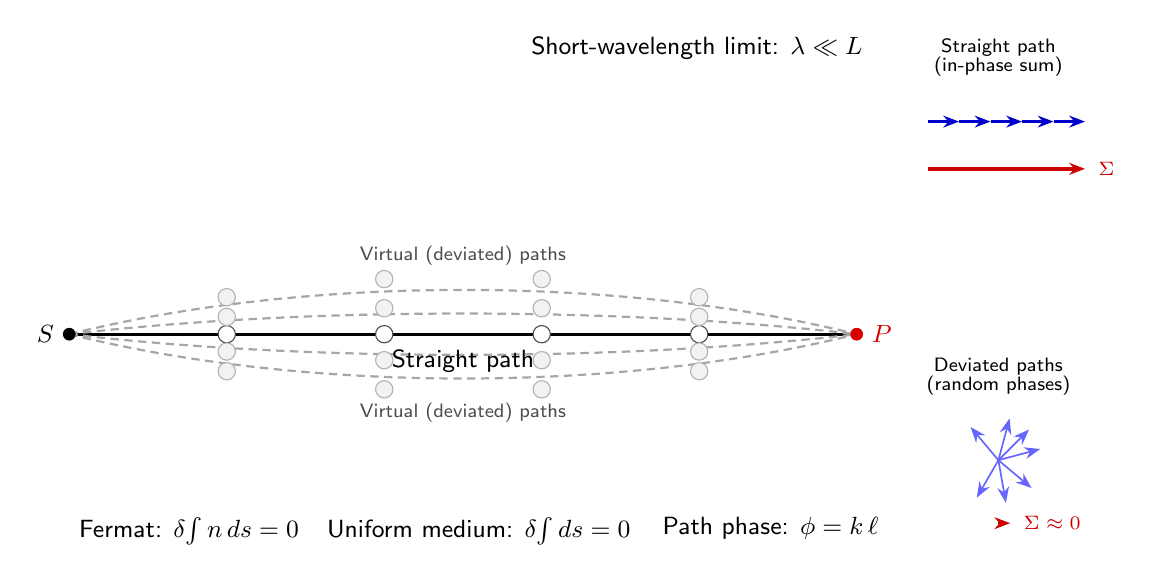
\begin{tikzpicture}[
    >={Stealth[length=2mm]},
    font=\sffamily\small,
    phase/.style={circle,draw=gray!60,fill=gray!10,inner sep=0pt,minimum size=2.2mm},
    phaseStr/.style={circle,draw=black!70,fill=white,inner sep=0pt,minimum size=2.2mm},
    vec/.style={->,blue!80!black,thick},
    vecOff/.style={->,blue!60,semithick},
    devpath/.style={gray!70,densely dashed,thick}
]

% --- Source and detector ---
\coordinate (S) at (0,0);
\coordinate (P) at (10,0);

% --- Straight line path ---
\draw[black,very thick] (S) -- (P);

% --- Deviation (virtual) paths: two above, two below ---
% Arcs rising slightly (2nd order), all sharing S and P endpoints
\draw[devpath] (S) .. controls (3,0.35) and (7,0.35) .. (P);
\draw[devpath] (S) .. controls (3,0.75) and (7,0.75) .. (P);
\draw[devpath] (S) .. controls (3,-0.35) and (7,-0.35) .. (P);
\draw[devpath] (S) .. controls (3,-0.75) and (7,-0.75) .. (P);

% --- Huygens wavelet phase markers along straight path ---
\foreach \x in {2,4,6,8}{
    \node[phaseStr] at (\x,0) {};
}

% --- Phase markers along deviation paths (sampled at midish points) ---
% upper arc 1 (h=0.35)
\foreach \x/\y in {2/0.22,4/0.33,6/0.33,8/0.22}{ \node[phase] at (\x,\y) {}; }
% upper arc 2 (h=0.75)
\foreach \x/\y in {2/0.47,4/0.70,6/0.70,8/0.47}{ \node[phase] at (\x,\y) {}; }
% lower arc 1
\foreach \x/\y in {2/-0.22,4/-0.33,6/-0.33,8/-0.22}{ \node[phase] at (\x,\y) {}; }
% lower arc 2
\foreach \x/\y in {2/-0.47,4/-0.70,6/-0.70,8/-0.47}{ \node[phase] at (\x,\y) {}; }

% --- Endpoints ---
\fill[black] (S) circle (2.3pt);
\fill[red!85!black] (P) circle (2.3pt);
\node[left=2pt of S] {$S$};
\node[right=2pt of P] {\textcolor{red!85!black}{$P$}};

% --- Straight path label ---
\node[below=1pt] at (5,-0.05) {Straight path};

% --- Label deviation paths ---
\node[gray!60!black,font=\sffamily\scriptsize] at (5,1.0) {Virtual (deviated) paths};
\node[gray!60!black,font=\sffamily\scriptsize] at (5,-1.0) {Virtual (deviated) paths};

% --- Short-wavelength limit annotation ---
\node[anchor=north east,font=\sffamily\small] at (10.2,3.9) {Short-wavelength limit: $\lambda \ll L$};

% --- Phase-sum diagrams ---
% Box on upper right: coherent sum (straight path) --> long resultant
\begin{scope}[shift={(11.8,2.2)}]
    \node[anchor=south,font=\sffamily\scriptsize] at (0,1.2) {Straight path};
    \node[anchor=south,font=\sffamily\scriptsize] at (0,0.95) {(in-phase sum)};
    % Parallel arrows stacked head-to-tail along +x
    \draw[vec] (-0.9,0.5) -- (-0.5,0.5);
    \draw[vec] (-0.5,0.5) -- (-0.1,0.5);
    \draw[vec] (-0.1,0.5) -- (0.3,0.5);
    \draw[vec] (0.3,0.5) -- (0.7,0.5);
    \draw[vec] (0.7,0.5) -- (1.1,0.5);
    % Resultant below
    \draw[->,red!80!black,ultra thick] (-0.9,-0.1) -- (1.1,-0.1);
    \node[anchor=west,red!80!black,font=\sffamily\scriptsize] at (1.15,-0.1) {$\Sigma$};
\end{scope}

% Box on lower right: incoherent sum (deviated paths) --> small resultant
\begin{scope}[shift={(11.8,-1.6)}]
    \node[anchor=south,font=\sffamily\scriptsize] at (0,0.95) {Deviated paths};
    \node[anchor=south,font=\sffamily\scriptsize] at (0,0.70) {(random phases)};
    % Arrows at varied angles from common origin
    \coordinate (O) at (0,0);
    \draw[vecOff] (O) -- ++(15:0.55);
    \draw[vecOff] (O) -- ++(75:0.55);
    \draw[vecOff] (O) -- ++(-40:0.55);
    \draw[vecOff] (O) -- ++(130:0.55);
    \draw[vecOff] (O) -- ++(-80:0.55);
    \draw[vecOff] (O) -- ++(45:0.55);
    \draw[vecOff] (O) -- ++(-120:0.55);
    % tiny resultant
    \draw[->,red!80!black,thick] (0,-0.8) -- (0.15,-0.8);
    \node[anchor=west,red!80!black,font=\sffamily\scriptsize] at (0.2,-0.8) {$\Sigma \approx 0$};
\end{scope}

% --- Formula labels along bottom ---
\node[anchor=north west,font=\sffamily\small] at (0,-2.2)
    {Fermat: $\delta\!\int n\,ds = 0$};
\node[anchor=north,font=\sffamily\small] at (5.2,-2.2)
    {Uniform medium: $\delta\!\int ds = 0$};
\node[anchor=north east,font=\sffamily\small] at (10.4,-2.2)
    {Path phase: $\phi = k\,\ell$};

\end{tikzpicture}
\end{document}
